All the underlying installation instructions assume a Linux operating system. We assume standard tools and libraries like CMake, compilers- (C, C++ and Fortran), CUDA/HIP (in case of GPU architectures), MPI, and math(BLAS-LAPACK) libraries are pre-installed. Most high-performance computers would have the latest version of these libraries in the default environment. However, in many cases you would have to use \href{http://modules.sourceforge.net/}{Environment Modules} to set the correct environment variables for the above and compilation tools like \href{http://www.cmake.org/}{CMake}. For example, on one of the high-performance computers (UMICH Greatlakes) we develop and test the \dftfe{} code, we can use the following commands to set the desired environment variables
\begin{verbatim}
$ module load cmake/3.18.2
$ module load gcc/8.2.0
$ module load openmpi/3.1.4
$ module load mkl/2018.0.4
$ module load cuda/11.0.2 (if installing for NVIDIA GPUs)
$ module load rocm/5.1.0 (if installing for AMD GPUs)
\end{verbatim}
%In the above mpilibrary denotes the MPI library you are using in your system(for eg: openmpi, mpich or intel-mpi). 
Note the above are shown only as an example. We strongly recommend using the latest stable version of compilers-(C, C++ and Fortran), CUDA/HIP, MPI and math libraries available on your high-performance computer. DFT-FE's installation requires also the following minimum versions of the above compilers and libraries:
\begin{itemize}
    \item CMake 3.17.0
    \item GCC 8.2.0
    \item CUDA 11.0.2/ ROCm (if installing for NVIDIA / AMD GPUs)
\end{itemize}
\textcolor{red}{\bf We currently do not support Intel compilers due to a compilation issue of the deal.II library. Please use GNU compilers only.} Further, if version of CMake greater than 3.17.0 is not available on your machine please install latest version from here \href{http://www.cmake.org/}{CMake} or use pre-installed binaries most appropriate for your machine.

\subsection{Compiling and installing external libraries}
\dftfe{} is primarily based on the open source finite element library \href{http://www.dealii.org/}{deal.II}, through which external dependencies
on \href{http://p4est.org/}{p4est} and BLAS-LAPACK are set. The other required external libraries, which are
not interfaced via deal.II are \href{http://www.alglib.net/}{ALGLIB}, \href{http://www.tddft.org/programs/libxc/}{Libxc}, \href{https://atztogo.github.io/spglib/}{spglib}, \href{http://www.xmlsoft.org/}{Libxml2} and \href{https://elpa.mpcdf.mpg.de/}{ELPA} (ELPA requires \href{http://www.netlib.org/scalapack/}{ScaLAPACK}). DFT-FE also optionally links to \href{https://www.mcs.anl.gov/petsc/}{PETSc} (via deali.II), \href{http://slepc.upv.es/}{SLEPc} (via deali.II) and to \href{https://developer.nvidia.com/nccl}{nccl} (for GPU compilation). The optional dependencies of PETSc and SLEPc are only required for all-electron calculations using DFT-FE, which uses the more stable Gram-Schmidt orthogonalization routine instead of the default Cholesky-Gram-Schmidt orthognalization. For pseudopotential calculations, PETSc and SLEPc dependencies are not required as the default Cholesky-Gram-Schmidt orthogonalization is very robust. \dftfe{} can also be linked to \href{https://github.com/awvwgk/simple-dftd3}{simple-dftd3} and \href{https://github.com/dftd4/dftd4}{dftd4} in order to provide support for the dftd family of dispersion corrections by Grimme et. al.. Below, we give brief installation instructions for each of the above libraries.
\subsubsection{Instructions for dependencies: ALGLIB, Libxc, spglib, Libxml2, ScaLAPACK, ELPA, p4est and nccl (nccl is optional)}
\begin{enumerate}
	\item   {\bf ALGLIB}: Used by \dftfe{} for spline fitting for various radial data. Download the current release of the Alglib free C++ edition from \url{http://www.alglib.net/download.php}. After downloading and unpacking, go to \verb|cpp/src|, and create a shared library using a C++ compiler. For example, using GCC compiler do
\begin{verbatim}
$ g++ -c -fPIC -O2 *.cpp
$ g++ *.o -shared -o libAlglib.so
\end{verbatim}
\item {\bf Libxc}: Used by \dftfe{} for exchange-correlation functionals. Download the current release from \url{http://www.tddft.org/programs/libxc/download/}, and do 
\begin{verbatim}
$ ./configure --prefix=libxc_install_dir_path
              CC=c_compiler CXX=c++_compiler FC=fortran_compiler
	       CFLAGS="-O2 -fPIC" FCFLAGS="-O2 -fPIC" CXXFLAGS="-O2 -fPIC"
     
$ make
$ make install
\end{verbatim}
Do not forget to replace \verb|libxc_install_dir_path| by some appropriate path on your file system and make sure that you have write permissions. Also replace \verb|c_compiler, c++_compiler| and \verb|fortran_compiler| with compilers on your system.

\item {\bf spglib}: Used by \dftfe{} to find crystal symmetries. To install spglib, first obtain the development version of spglib from their github repository by
\begin{verbatim}
$ git clone https://github.com/atztogo/spglib.git	
\end{verbatim}	
and next follow the ``Compiling using cmake'' installation procedure described in \url{https://atztogo.github.io/spglib/install.html}.   	
We recommend using the ccmake gui interface for the installation and also use appropriate compiler for \verb|CMAKE_C_COMPILER|.

\item {\bf Libxml2}: Libxml2 is used by \dftfe{} to read \verb|.xml| files. Most likely, Libxml2 might be already installed in the high-performance computer you are working with. It is usually installed in the default locations like \verb|/usr/lib64| (library path which contains \verb|.so| file for Libxml2, something like \verb|libxml2.so.2|) and \verb|/usr/include/libxml2| (include path). 

Libxml2 can also be installed by doing (Do not use these instructions if you have already have Libxml2 on your system)
\begin{verbatim}
$ git clone https://gitlab.gnome.org/GNOME/libxml2.git
$ ./autogen.sh --prefix=Libxml_install_dir_path
$ make
$ make install 
\end{verbatim}
There might be errors complaining that it can not create regular file libxml2.py in /usr/lib/python2.7/site-packages, but that should not matter.

\item {\bf ScaLAPACK}: ScaLAPACK library is used by DFT-FE via ELPA for its parallel linear algebra routines involving dense matrices, as well being a dependency for ELPA. \textcolor{red}{\bf If Intel MKL math library is available, please skip this step, as the ScaLAPACK libraries therein can be used directly.} If Intel MKL math library is not available, Netlib ScaLAPACK \url{http://www.netlib.org/scalapack/} needs to be installed using the instructions below. Download the current release version (2.2.0) from \url{http://www.netlib.org/scalapack/#\_software}, and build a shared library (use \verb|BUILD_SHARED_LIBS=ON|, \verb|BUILD_STATIC_LIBS=OFF| and \verb|BUILD_TESTING=OFF|) installation of ScaLAPACK using cmake. We recommend using the ccmake gui interface for the installation.  Further, use the appropriate compilers for \verb|CMAKE_C_COMPILER| and \verb|CMAKE_FORTRAN_COMPILER|, and also use \verb|-fPIC| flag for \verb|CMAKE_C_FLAGS| and \verb|-fPIC -fallow-argument-mismatch| for \verb|CMAKE_Fortran_FLAGS|. For best performance, ScaLAPACK must be linked to optimized BLAS-LAPACK libraries by using\\ \verb|USE_OPTIMIZED_LAPACK_BLAS=ON|, and providing external paths to BLAS-LAPACK libraries (MKL, OpenBlas, ESSL etc.) during the cmake configuration. 
%Alternatively one can also use the python based installer~\url{http://www.netlib.org/scalapack/scalapack_installer.tgz} for Linux.

\item {\bf ELPA}: ELPA library is used by DFT-FE for its parallel linear algebra routines involving dense matrices. ELPA requires the ScaLAPACK library (see above) as a dependency. Download the latest version elpa-2022.11.001 from \url{https://elpa.mpcdf.mpg.de/software/} and follow the installation instructions in there. Example of ELPA installation on UMICH Greatlakes supercomputer with GNU compiler, Open MPI library, and Intel MKL math library:
\begin{verbatim}
$ cd elpaDir
$ mkdir build
$ cd build
$ ../configure --enable-openmp FC=mpif90 CC=mpicc CXX=mpicxx 
FCFLAGS="-fopenmp -O2 -march=native" CFLAGS="-fopenmp -O2 -march=native" 
CXXFLAGS="-fopenmp -O2 -march=native" --prefix=elpa_install_path
SCALAPACK_LDFLAGS=" -L${MKLROOT}/lib/intel64 -lmkl_scalapack_lp64
-Wl,--no-as-needed -lmkl_intel_lp64
-lmkl_gnu_thread -lmkl_core -lmkl_blacs_openmpi_lp64 -lgomp -lpthread -lm -ldl" 
SCALAPACK_FCFLAGS="-L${MKLROOT}/lib/intel64 -lmkl_scalapack_lp64
-Wl,--no-as-needed -lmkl_gf_lp64 -lmkl_gnu_thread -lmkl_core
-lmkl_blacs_openmpi_lp64 -lgomp -lpthread -lm -ldl"
$ make -j 4
$ make install
\end{verbatim}
The MKL paths and linker flags were obtained with the help of \href{https://software.intel.com/en-us/articles/intel-mkl-link-line-advisor}{Intel MKL Link Line Advisor} for GNU Fortran compiler (Note the usage of \verb|-lmkl_gf_lp64| flag above).\\ 

If the machine of interest has NVIDIA/AMD GPUs and CUDA/ROCm compiler, ELPA can take advantage of GPUs. For example on OLCF Summit GPU nodes, we use the following configure line
\begin{verbatim}
../configure CXX=mpic++ FC=mpif90 CC=mpicc 
CXXFLAGS="-O2 -fPIC -mcpu=power9 -mvsx -maltivec"
FCFLAGS="-O2 -fPIC -mcpu=power9 -mvsx -maltivec" 
CFLAGS="-O2 -fPIC -mcpu=power9 -mvsx -maltivec"
--enable-nvidia-gpu --with-NVIDIA-GPU-compute-capability="sm_70" 
--enable-gpu-streams=nvidia --with-cuda-path="$OLCF_CUDA_ROOT"
--with-cuda-sdk-path="$OLCF_CUDA_ROOT" 
--prefix=elpa_install_path 
LDFLAGS="-L$scalapack_lib_path -lscalapack  
-L$OLCF_ESSL_ROOT/lib64 -lessl 
-L$OLCF_NETLIB_LAPACK_ROOT/lib64 -llapack 
-L$OLCF_OPENBLAS_ROOT/lib -lopenblas"
--disable-sse --disable-sse-assembly --disable-avx 
--disable-avx2 --disable-avx512 --enable-c-tests=no --enable-cpp-tests=no
--enable-option-checking=fatal --enable-shared 
\end{verbatim}


We provice another ELPA installation example on OLCF Crusher nodes with AMD GPUs and ROCm compiler:
\begin{verbatim}
../configure CXX=hipcc CC=hipcc FC=ftn 
FCFLAGS="-march=znver3 -O2 -fPIC" 
CFLAGS="-march=znver3 -fPIC -O2 -I${ROCM_PATH}/include 
-I${ROCM_PATH}/hip/include -I${ROCM_PATH}/hipcub/include
-I${ROCM_PATH}/rocblas/include  --amdgpu-target=gfx90a
-I${MPICH_DIR}/include" CXXFLAGS="-march=znver3 -std=c++14 
-I${ROCM_PATH}/include -fPIC -O2 -I${ROCM_PATH}/hip/include 
-I${ROCM_PATH}/hipcub/include -I${ROCM_PATH}/rocblas/include 
--amdgpu-target=gfx90a -I${MPICH_DIR}/include" --enable-amd-gpu
--enable-gpu-streams=amd --prefix=elpa_install_path
LIBS="-L${ROCM_PATH}/lib -lamdhip64 -L${ROCM_PATH}/rocblas/lib 
-lrocblas -L${MPICH_DIR}/lib -lmpi -L${CRAY_MPICH_ROOTDIR}/gtl/lib -lmpi_gtl_hsa 
-L$scalapack_lib_path -lscalapack
-L/sw/crusher/spack-envs/base/opt/cray-sles15-zen3/gcc-11.2.0/openblas-0.3.17-fip547hyhcrii2xgj5rmge3oyxgnfhkp/lib -lopenblas 
-L$netlib_lapack_lib_path -llapack" 
--disable-sse --disable-sse-assembly --disable-avx --disable-avx2 
--disable-avx512 --enable-c-tests=no --enable-option-checking=fatal
--enable-shared --enable-cpp-tests=no --enable-hipcub
\end{verbatim}


Note the use of LDFLAGS instead of SCALAPACK\_LDFLAGS and SCALAPACK\_FCFLAGS, since we are using netlib ScaLAPACK instead of Intel MKL ScaLAPACK in the above. Also note use of
\begin{verbatim}
    --disable-sse --disable-sse-assembly --disable-avx --disable-avx2 --disable-avx512
\end{verbatim} 
above. \textcolor{red}{\bf Some or all of these options may be required for systems without Intel CPUs such as IBM Power and AMD Epyc processors depending on what they support.} Finally, we remark that to avoid errors during ELPA configuration step, please export the library paths of ScaLAPACK and blas libraries, for example:
\begin{verbatim}
export LD_LIBRARY_PATH=$LD_LIBRARY_PATH:$blas_lib_path

export LD_LIBRARY_PATH=$LD_LIBRARY_PATH:$netlib_lapack_lib_path

export LD_LIBRARY_PATH=
$LD_LIBRARY_PATH:$ROCM_PATH/lib:$ROCM_PATH/hip/lib:$ROCM_PATH/lib:$ROCM_PATH/rocblas/lib
\end{verbatim}

\item   {\bf p4est}: This library is used by deal.II to create and distribute finite-element meshes across multiple processors. Download the v2.2 tarball of p4est from \url{https://github.com/p4est/p4est.github.io/raw/master/release/p4est-2.2.tar.gz}. Next download the \verb|p4est-setup.sh| script from \url{https://raw.githubusercontent.com/dftfeDevelopers/dftfe/manual/p4est-setup.sh}. Use the script to automatically compile and install a debug and optimized version of p4est by doing
\begin{verbatim}
$ chmod u+x p4est-setup.sh
$ ./p4est-setup.sh p4est-x-y-z.tar.gz p4est_install_dir_path
\end{verbatim}

%Also download the script from \url{https://github.com/dftfeDevelopers/dftfe/raw/manual/p4est-setup.sh} if using Intel compilers, or from \url{https://dealii.org/developer/external-libs/p4est.html} if using GCC compilers. Use the script to automatically compile and install a debug and optimized version of p4est by doing

\item {\bf nccl/rccl (optional)}: nccl (CUDA) and rccl (ROCm) libraries are optional dependency for DFT-FE for optimal GPU Direct MPI collective communication calls. This library is recommended for running very large system sizes (greater than 20,000 electrons) on GPUs using DFT-FE. Caution: nccl/rccl library requires appropriate hardware support for GPU Direct MPI communication and GPU Aware MPI library. To install nccl/rccl, use the appropriate release version (corresponding to the CUDA/ROCm compiler version) from \url{https://github.com/NVIDIA/nccl} (CUDA) \url{https://github.com/ROCmSoftwarePlatform/rccl} (ROCm) and follow installation instructions therein.

\end{enumerate}


\subsubsection{Instructions for deal.II}
Assuming the above p4est dependency is installed, we now briefly discuss the steps to compile and install deal.II library linked with the above dependencies. You need to install two variants of the deal.II library-- one variant linked with real scalar type PETSc and SLEPc installations, and the other variant linked with complex scalar type PETSc and SLEPc installations. 

\begin{enumerate}

\item Obtain the customized version of deal.II library via
\begin{verbatim}
$ git clone -b dealiiCustomizedCUDARelease https://github.com/dftfeDevelopers/dealii.git
\end{verbatim}

\item In addition to requiring C, C++ and Fortran compilers, MPI library, and CMake, deal.II additionally requires BOOST library. If not found externally, cmake will resort to the bundled BOOST that comes along with deal.II. Based on our experience, we recommend to use the deal.II's bundled boost (enforced by unsetting/unloading external BOOST library environment paths) to avoid compilation issues. Please do not install deal.II with GPU support as that is not needed by DFT-FE. Further, when installing deal.II for (DFT-FE with GPU support), one must use \verb|-DDEAL_II_ALLOW_PLATFORM_INTROSPECTION=OFF| to avoid compilation failure of DFT-FE.

\item
\begin{verbatim}
$ mkdir build
$ cd build
$ cmake -DCMAKE_INSTALL_PREFIX=dealii_install_dir_path
        otherCmakeOptions ../deal.II
$ make -j 8        
$ make install
\end{verbatim}
{\bf ``otherCmakeOptions'' include} the following options for CPU installation:
\begin{verbatim}
-DCMAKE_CXX_STANDARD=17
-DCMAKE_C_COMPILER=c_compiler
-DCMAKE_CXX_COMPILER=cxx_compiler
-DCMAKE_Fortran_COMPILER=fortran_compiler
-DMPI_C_COMPILER=mpi_c_compiler_wrapper
-DMPI_CXX_COMPILER=mpi_cxx_compiler_wrapper
-DMPI_Fortran_COMPILER=mpi_fortran_compiler_wrapper
-DCMAKE_CXX_FLAGS=cxx_flags
-DCMAKE_C_FLAGS=c_flags
-DDEAL_II_WITH_MPI=ON -DDEAL_II_WITH_64BIT_INDICES=ON
-DDEAL_II_WITH_P4EST=ON -DP4EST_DIR=p4est_install_dir_path
-DDEAL_II_WITH_LAPACK=ON
-DLAPACK_DIR=lapack_dir_paths (both BLAS and LAPACK directory paths)
-DLAPACK_FOUND=true
-DLAPACK_LIBRARIES=lapack_lib_paths (both BLAS and LAPACK library paths)
-DDEAL_II_WITH_TBB=OFF
-DDEAL_II_WITH_TASKFLOW=OFF
-DDEAL_II_COMPONENT_EXAMPLES=OFF
-DDEAL_II_FORCE_BUNDLED_BOOST=ON
\end{verbatim}



\end{enumerate}	
 For more information about installing deal.II library refer to \url{https://dealii.org/developer/readme.html}. We also provide here an example of deal.II installation, which we did on UMICH Greatlakes supercomputer with GNU compiler, Open MPI library, and Intel MKL math library
\begin{verbatim}
$ mkdir build
$ cd build
$ cmake
-DCMAKE_CXX_STANDARD=17
-DCMAKE_C_COMPILER=gcc 
-DCMAKE_CXX_COMPILER=g++
-DCMAKE_Fortran_COMPILER=gfortran
-DMPI_C_COMPILER=mpicc 
-DMPI_CXX_COMPILER=mpicxx 
-DMPI_Fortran_COMPILER=mpif90
-DCMAKE_CXX_FLAGS="-march=native -std=c++17"
-DCMAKE_C_FLAGS="-march=native -std=c++17"
-DDEAL_II_CXX_FLAGS_RELEASE="-O2"
-DDEAL_II_COMPONENT_EXAMPLES=OFF
-DDEAL_II_WITH_MPI=ON
-DDEAL_II_WITH_64BIT_INDICES=ON
-DDEAL_II_WITH_TBB=OFF
-DDEAL_II_WITH_TASKFLOW=OFF 
-DDEAL_II_FORCE_BUNDLED_BOOST=ON
-DDEAL_II_WITH_P4EST=ON 
-DP4EST_DIR=p4est_install_path 
-DDEAL_II_WITH_LAPACK=ON -DLAPACK_DIR="${MKLROOT}/lib/intel64"
-DLAPACK_FOUND=true
-DLAPACK_LIBRARIES="-L${MKLROOT}/lib/intel64
-Wl,--no-as-needed -lmkl_intel_lp64
-lmkl_gnu_thread -lmkl_core -lgomp -lpthread -lm
-ldl" -DLAPACK_INCLUDE_DIRS="-I${MKLROOT}/include" 
-DCMAKE_INSTALL_PREFIX=dealii_install_path ../dealii
$ make -j 8
$ make install
\end{verbatim}
The values for \verb|-DLAPACK_DIR|,\verb|-DLAPACK_LIBRARIES| and \verb|-DLAPACK_LINKER_FLAGS| were obtained with the help of \href{https://software.intel.com/en-us/articles/intel-mkl-link-line-advisor}{Intel MKL Link Line Advisor} for GNU C++ compiler (cf. Fig.~\ref{fig:intelmkl}).\\ 
\begin{figure}[htp]
    \centering
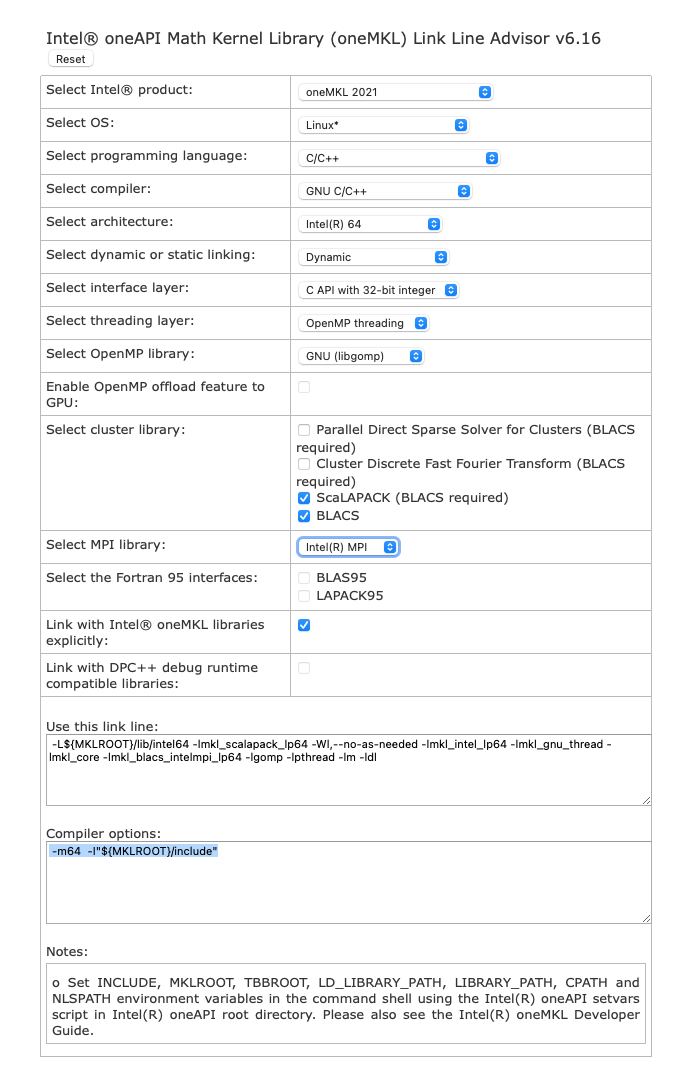
\includegraphics[scale=0.4]{intelmklLineAdvisorExampleNew.png}
    \caption{Example usage of Intel MKL line advisor. Use the options in the ``link line'' generated by the line advisor tool. Please note to change ``intelmpi'' in ``-lmkl\_blacs\_intelmpi\_lp64'' to ``openmpi'' if using openmpi MPI library.}
    \label{fig:intelmkl}
\end{figure}

%Note that in the above procedure one is installing the development version of deal.II library and this version is continuously updated by deal.II developers, which can sometimes lead to installation issues on certain compilers. If you face any issues during the installation procedure of deal.II development version as explained above, you may alternatively obtain the current release version of deal.II by downloading and unpacking the .tar.gz file from \url{https://www.dealii.org/download.html} and following the same procedure as above. If you still face installation issues, and/or if you have any questions about the deal.II installation, please contact the deal.II developers at \href{https://groups.google.com/d/forum/dealii}{deal.II mailing lists}.\\



\subsubsection{Instructions for simple-dftd3 and dftd4}

\begin{enumerate}
	\item   {\bf simple-dftd3}: Used by \dftfe{} to provide dftd3 corrections to energy, force and stress. Download the current release (0.6.0 at the time of writing) of simple-dftd3 from \url{https://github.com/awvwgk/simple-dftd3/releases}. After downloading and unpacking, use cmake to build the library. For example, using GNU compiler and Intel MKL for BLAS, do
\begin{verbatim}
$ FC=gfortran cmake -B _build 
-DBLAS_LIBRARIES="-L${MKLROOT}/lib/intel64 
-Wl,--no-as-needed -lmkl_gf_lp64 
-lmkl_gnu_thread -lmkl_core -lgomp 
-lpthread -lm -ldl" 
-DCMAKE_INSTALL_PREFIX=simple_dftd3_install_path
$ cmake --build _build
$ cmake --install _build 
\end{verbatim}
	\item   {\bf dftd4}: Used by \dftfe{} to provide dftd4 corrections to energy, force and stress. Download the current release (3.6.0 at the time of writing) of dftd4 from \url{https://github.com/dftd4/dftd4/releases}. After downloading and unpacking, use cmake to build the library. For example, using GNU compiler and Intel MKL for BLAS and LAPACK, do
\begin{verbatim}
$ cd dftd4-3.6.0
$ mkdir build 
$ cd build
$ cmake -DCMAKE_Fortran_COMPILER=gfortran
        -DCMAKE_C_COMPILER=gcc
        -DBLAS_LIBRARIES="-L${MKLROOT}/lib/intel64 -Wl,--no-as-needed
        -lmkl_intel_lp64 -lmkl_gnu_thread -lmkl_rt -lmkl_core -lgomp 
        -lpthread -lm -ldl" 
        -DLAPACK_LIBRARIES="-L${MKLROOT}/lib/intel64 -Wl,--no-as-needed -lmkl_intel_lp64
        -lmkl_gnu_thread -lmkl_rt -lmkl_core 
        -lgomp -lpthread -lm -ldl"
        -DBUILD_SHARED_LIBS=ON 
        -DCMAKE_INSTALL_PREFIX=dftd4_install_path
        -DWITH_OpenMP=OFF
        ..
$ make -j16
$ make install
\end{verbatim}
\end{enumerate}
The values for \verb|-DBLAS_LIBRARIES| and \verb|-DLAPACK_LIBRARIES| were obtained with the help of \href{https://software.intel.com/en-us/articles/intel-mkl-link-line-advisor}{Intel MKL Link Line Advisor} for GNU fortran compiler.\\ 

\subsection{Obtaining and Compiling \dftfe{}}\label{sec:dftfeinstall}
Assuming that you have already installed the above external dependencies, next follow the steps below to obtain and compile \dftfe{}.
\begin{enumerate}
\item Obtain the source code of the current release of \dftfe{} with all current patches using \href{https://git-scm.com/}{Git}:
\begin{verbatim}
$ git clone -b release1.0 https://github.com/dftfeDevelopers/dftfe.git
$ cd dftfe
\end{verbatim}
Do \verb|git pull| in the \verb|dftfe| directory any time to obtain new patches that have been added since your \verb|git clone| or last \verb|git pull|.
If you are not familiar with Git, you may download the current release tarball from the \href{https://sites.google.com/umich.edu/dftfe/download}{Downloads} page in our website, but downloading via Git is recommended to avail new patches seamlessly. 


%{\bf Obtaining previous releases:} (Skip this part if you are using the current release version)
%\begin{enumerate}
%\item
%\begin{verbatim}
%$ git clone https://github.com/dftfeDevelopers/dftfe.git 
%$ cd dftfe
%\end{verbatim}

%\item To get the list of all release tags (current and previous releases) do
%\begin{verbatim}
%$ git tag -l
%\end{verbatim}

%\item
%Choose the desired release tag name and do
%\begin{verbatim}
%$ git checkout tags/<tag_name> 
%\end{verbatim}
%\end{enumerate}
%Alternatively, you could download the appropriate tarball from \href{https://github.com/dftfeDevelopers/dftfe/releases}{github-releases}.

\item Set paths to external libraries (deal.II, ALGLIB, Libxc, spglib, Libxml2, and ELPA), C++ compiler, and C++ compiler flags in \verb|setupUser.sh|, which is a script to compile \dftfe~using cmake. nccl library can also be optionally provided in case of GPU compilation. If compiling only for CPUs, set the following to OFF
\begin{verbatim}
withGPU=OFF
withDCCL=OFF
\end{verbatim}
For GPU compilation, \verb|withGPU|, \verb|gpuLang|, and \verb|gpuVendor| should be set \verb|ON|, \verb|"cuda"/"hip"| and \verb|"nvidia"/"amd"| respectively. Also appropriate C++ compiler, device (denoting GPU) compilation and architecture flags must be passed to access CUDA/HIP compiler for device code compilation. \textcolor{red}{\bf CAUTION! GPU enabled DFT-FE compilation must only be run on machines with GPU access.} 
\item To compile \dftfe{}, first create a build directory anywhere on your machine. Next from inside the build directory do
\begin{verbatim}
$ bash $dftfe_source/setupUser.sh
\end{verbatim} 
Please use the full directory path for \verb|$dftfe_source| above. Also note that sometimes compilation on login node can crash due to insufficient memory. In those cases, we recommend using an interactive job if available on your computing cluster.

\item If compilation is successful, the following executables will be created:
\begin{verbatim}
$dftfe_build_dir/release/real/dftfe
$dftfe_build_dir/release/complex/dftfe
\end{verbatim}

\item
To compile \dftfe{} in debug mode (much slower but useful for debugging), set \verb|build_type=Debug| in \verb|setupUser.sh| and do:
\begin{verbatim}
$ bash $dftfe_source/setupUser.h
\end{verbatim}
which will create the following debug mode executables:
\begin{verbatim}
$dftfe_build_dir/debug/real/dftfe
$dftfe_build_dir/debug/complex/dftfe
\end{verbatim}
\end{enumerate}



\subsection{Optional PETSc, SLEPc, deal.II and \dftfe~ installation instructions for all-electron calculations using DFT-FE}
Users can ignore this section if only interested in pseudopotential calculations. The optional dependencies of PETSc and SLEPc are only required for all-electron calculations using DFT-FE, which uses the more stable Gram-Schmidt orthogonalization routine instead of the default Cholesky-Gram-Schmidt orthognalization. 
    
\begin{enumerate}
\item {\bf PETSc}: PETSc is a parallel linear algebra library. \dftfe{} with PETSc and SLEPc dependencies needs two variants of the PETSc installation---one with real scalar type and the another with complex scalar type. Also both the installation variants must have 64-bit indices and optimized mode enabled during the installation. To install PETSc, first download the current release (3.15.0 or later) tarball from \url{https://www.mcs.anl.gov/petsc/download/index.html}, unpack it, and follow the installation instructions in \url{https://www.mcs.anl.gov/petsc/documentation/installation.html}. 
	
Below, we show an example installation for the real scalar type variant. 
This example should be used only as a reference.
\begin{verbatim}
$ ./configure --prefix=petscReal_install_dir_path --with-debugging=no 
              --with-64-bit-indices=true --with-cc=c_compiler
              --with-cxx=c++_compiler --with-fc=fortran_compiler
              --with-blas-lapack-lib=(optimized BLAS-LAPACK library path) 
              CFLAGS=c_compilter_flags CXXFLAGS=c++_compiler_flags
	              FFLAGS=fortran_compiler_flags

$ make PETSC_DIR=prompted by PETSc 
       PETSC_ARCH=prompted by PETSc

$ make PETSC_DIR=prompted by PETSc 
       PETSC_ARCH=prompted by PETSc
       install
\end{verbatim}
For the complex installation variant, unpack a fresh PETSc directory (required) from the tarball and repeat the above steps with the only changes being adding  \verb|--with-scalar-type=complex| and \verb|--with-fortran-kernels=true| to the configuration step (\verb|./configure|) as well as providing a new installation path to \verb|--prefix|. Below we provide example configure lines for real and complex versions on UMICH Greatlakes supercomputer with GNU compiler, Open MPI library, and Intel MKL math library:
\begin{verbatim}
./configure --prefix=petsc_real_install_path --with-debugging=no 
--with-64-bit-indices=true --with-cc=mpicc --with-cxx=mpicxx 
--with-fc=mpif90 --with-blas-lapack-lib="-Wl,--start-group
${MKLROOT}/lib/intel64/libmkl_intel_lp64.a 
${MKLROOT}/lib/intel64/libmkl_gnu_thread.a 
${MKLROOT}/lib/intel64/libmkl_core.a -Wl,--end-group -lgomp -lpthread -lm -ldl"
CFLAGS="-O2" CXXFLAGS="-O2" FFLAGS="-O2"

./configure --prefix=petsc_complex_install_path --with-debugging=no
--with-64-bit-indices=true --with-cc=mpicc --with-cxx=mpicxx
--with-fc=mpif90 --with-fortran-kernels=true --with-scalar-type=complex
--with-blas-lapack-lib="-Wl,--start-group 
${MKLROOT}/lib/intel64/libmkl_intel_lp64.a ${MKLROOT}/lib/intel64/libmkl_gnu_thread.a
${MKLROOT}/lib/intel64/libmkl_core.a -Wl,--end-group -lgomp -lpthread -lm -ldl"
CFLAGS="-O2" CXXFLAGS="-O2" FFLAGS="-O2"
\end{verbatim}

\item {\bf SLEPc}: The SLEPc library is built on top of PETSc, and it is used in DFT-FE for Gram-Schmidt Orthogonalization. To install SLEPc, first download the current release (3.15.0 or later) tarball from \url{http://slepc.upv.es/download/}, and then follow the installation procedure described in \url{http://slepc.upv.es/documentation/instal.htm}. {\bf Important: } SLEPc installation requires PETSc to be installed first. You also need to create two separate SLEPc installations- one for PETSc installed with \\\verb|--with-scalar-type=real|, and the second for PETSc installed with \verb|--with-scalar-type=complex|. 
	
For your reference you provide here an example installation of SLEPc for real scalar type
\begin{verbatim}
$ export PETSC_DIR=petscReal_install_dir_path
$ unset PETSC_ARCH
$ cd downloaded_slepc_dir
$ ./configure --prefix=slepcReal_install_dir_path
$ make
$ make install
\end{verbatim}


\item {\bf deal.II}: Assuming PETSc and SLEPc are installed, we now briefly discuss the steps to compile and install deal.II library linked with the above dependencies. You need to install two variants of the deal.II library---one variant linked with real scalar type PETSc and SLEPc installations, and the other variant linked with complex scalar type PETSc and SLEPc installations. 

\begin{verbatim}
$ mkdir buildReal
$ cd buildReal
$ cmake -DCMAKE_INSTALL_PREFIX=dealii_petscReal_install_dir_path
        otherCmakeOptions ../deal.II
$ make install
\end{verbatim}
{\bf ``otherCmakeOptions'' include} the following options
\begin{verbatim}
-DCMAKE_C_COMPILER=c_compiler
-DCMAKE_CXX_COMPILER=cxx_compiler
-DCMAKE_Fortran_COMPILER=fortran_compiler
-DMPI_C_COMPILER=mpi_c_compiler_wrapper
-DMPI_CXX_COMPILER=mpi_cxx_compiler_wrapper
-DMPI_Fortran_COMPILER=mpi_fortran_compiler_wrapper
-DCMAKE_CXX_FLAGS=cxx_flags
-DCMAKE_C_FLAGS=c_flags
-DDEAL_II_WITH_MPI=ON -DDEAL_II_WITH_64BIT_INDICES=ON
-DDEAL_II_WITH_P4EST=ON -DP4EST_DIR=p4est_install_dir_path
-DDEAL_II_WITH_PETSC=ON -DPETSC_DIR=petscReal_install_dir_path 
-DDEAL_II_WITH_SLEPC=ON -DSLEPC_DIR=slepcReal_install_dir_path
-DDEAL_II_WITH_LAPACK=ON
-DLAPACK_DIR=lapack_dir_path 
-DLAPACK_FOUND=true 
-DLAPACK_LIBRARIES=lapack_lib_path
-DDEAL_II_WITH_TBB=OFF
-DDEAL_II_WITH_TASKFLOW=OFF
-DDEAL_II_COMPONENT_EXAMPLES=OFF
\end{verbatim}

\item {\bf DFT-FE}: Follow the same instructions as in Sec.~\ref{sec:dftfeinstall}, except to modify the \verb|setupUserPetsc.sh| script instead of the \verb|setupUser.sh|. In \verb|setupUserPetsc.sh|, in addition to updating the paths and flags as discussed in Sec~\ref{sec:dftfeinstall}, update the dealii installation paths from the previous step as follows:
\begin{verbatim}
dealiiPetscRealDir=dealii_petscReal_install_dir_path
dealiiPetscComplexDir=dealii_petscComplex_install_dir_path
\end{verbatim}
\end{enumerate}


\subsection{Important generic instructions}
\begin{itemize}
\item We strongly recommend to link to optimized BLAS-LAPACK library. If using Intel MKL for BLAS-LAPACK library, it is {\bf very important} to use \href{https://software.intel.com/en-us/articles/intel-mkl-link-line-advisor}{Intel MKL Link Line Advisor} to correctly link with Intel MKL for installations of PETSc, ScaLAPACK, ELPA, deal.II, and PETSc. To exploit performance benefit from threads, we recommend (strongly recommended for the new Intel Xeon Phi (KNL) and Skylake processors) linking to threaded versions of Intel MKL libraries by using the options ``threading layer'' and  ``OpenMP library'' in \href{https://software.intel.com/en-us/articles/intel-mkl-link-line-advisor}{Intel MKL Link Line Advisor}.

\item Use \verb|-fPIC| compiler flag for compilation of \dftfe{} and its dependencies, to prevent linking errors during \dftfe{} compilation.	

\item \textcolor{red}{\bf CAUTION! It is  highly recommended to compile deal.II, p4est, ScaLAPACK, ELPA, \dftfe, PETSc and SLEPc~ with the same compilers, same BLAS-LAPACK libraries (if applicable), and same MPI libraries. This prevents deal.II compilation issues, occurrence of run time crashes, and \dftfe{} performance degradation.}  
\end{itemize}
